%%%%%%%%%%%%%%%%%%%%%%%%%%%%%%%%%%%%%%%%%
% Programming/Coding Assignment
% LaTeX Template
%
% This template has been downloaded from:
% http://www.latextemplates.com
%
% Original author:
% Ted Pavlic (http://www.tedpavlic.com)
%
% Note:
% The \lipsum[#] commands throughout this template generate dummy text
% to fill the template out. These commands should all be removed when 
% writing assignment content.
%
% This template uses a Perl script as an example snippet of code, most other
% languages are also usable. Configure them in the "CODE INCLUSION 
% CONFIGURATION" section.
%
%%%%%%%%%%%%%%%%%%%%%%%%%%%%%%%%%%%%%%%%%

%----------------------------------------------------------------------------------------
%	PACKAGES AND OTHER DOCUMENT CONFIGURATIONS
%----------------------------------------------------------------------------------------

\documentclass{article}

\usepackage{fancyhdr} % Required for custom headers
\usepackage{lastpage} % Required to determine the last page for the footer
\usepackage{extramarks} % Required for headers and footers
\usepackage[usenames,dvipsnames]{color} % Required for custom colors
\usepackage{graphicx} % Required to insert images
\usepackage{listings} % Required for insertion of code
\usepackage{courier} % Required for the courier font
\usepackage{lipsum} % Used for inserting dummy 'Lorem ipsum' text into the template
\usepackage{epstopdf} % Convert Matlab figures to pdf
\usepackage{amsmath}
\usepackage{esint}
\usepackage{cancel}
\usepackage{amssymb}

% Margins
\topmargin=-0.45in
\evensidemargin=0in
\oddsidemargin=0in
\textwidth=6.5in
\textheight=9.0in
\headsep=0.25in

\linespread{1.1} % Line spacing

% Set up the header and footer
\pagestyle{fancy}
\lhead{\hmwkAuthorName} % Top left header
\chead{\hmwkClass\ (\hmwkClassInstructor): \hmwkTitle} % Top center head
\rhead{\firstxmark} % Top right header
\lfoot{\lastxmark} % Bottom left footer
\cfoot{} % Bottom center footer
\rfoot{Page\ \thepage\ of\ \protect\pageref{LastPage}} % Bottom right footer
\renewcommand\headrulewidth{0.4pt} % Size of the header rule
\renewcommand\footrulewidth{0.4pt} % Size of the footer rule

\setlength\parindent{0pt} % Removes all indentation from paragraphs

%----------------------------------------------------------------------------------------
%	CODE INCLUSION CONFIGURATION
%----------------------------------------------------------------------------------------

\definecolor{MyDarkGreen}{rgb}{0.0,0.4,0.0} % This is the color used for comments
\lstloadlanguages{Python} % Load Python syntax for listings, for a list of other languages supported see: ftp://ftp.tex.ac.uk/tex-archive/macros/latex/contrib/listings/listings.pdf
\lstset{language=Python, % Use Python
        frame=single, % Single frame around code
        basicstyle=\small\ttfamily, % Use small true type font
        keywordstyle=[1]\color{Blue}\bf, % Matlab functions bold and blue
        keywordstyle=[2]\color{Purple}, % Matlab function arguments purple
        keywordstyle=[3]\color{Blue}\underbar, % Custom functions underlined and blue
        identifierstyle=, % Nothing special about identifiers                                         
        commentstyle=\usefont{T1}{pcr}{m}{sl}\color{MyDarkGreen}\small, % Comments small dark green courier font
        stringstyle=\color{Purple}, % Strings are purple
        showstringspaces=false, % Don't put marks in string spaces
        tabsize=5, % 5 spaces per tab
        %
        % Put standard Python functions not included in the default language here
        morekeywords={rand,logrnd,var,mode,skewness,kurtosis},
        %
        % Put function parameters here
        morekeywords=[2]{on, off, interp},
        %
        % Put user defined functions here
        morekeywords=[3]{test},
       	%
        morecomment=[l][\color{Blue}]{...}, % Line continuation (...) like blue comment
        numbers=left, % Line numbers on left
        firstnumber=1, % Line numbers start with line 1
        numberstyle=\tiny\color{Blue}, % Line numbers are blue and small
        stepnumber=5 % Line numbers go in steps of 5
}

% Creates a new command to include a script, the first parameter is the filename of the script (without .m), the second parameter is the caption
\newcommand{\script}[5]{
\begin{itemize}
\item[]\lstinputlisting[caption=#2,label=#1,firstline=#3,lastline=#4,firstnumber=#5]{#1.py}
\end{itemize}
}

%----------------------------------------------------------------------------------------
%	DOCUMENT STRUCTURE COMMANDS
%	Skip this unless you know what you're doing
%----------------------------------------------------------------------------------------

% Header and footer for when a page split occurs within a problem environment
\newcommand{\enterProblemHeader}[1]{
\nobreak\extramarks{#1}{#1 continued on next page\ldots}\nobreak
\nobreak\extramarks{#1 (continued)}{#1 continued on next page\ldots}\nobreak
}

% Header and footer for when a page split occurs between problem environments (seems to be where listing the previous problem between problems is occurring)
\newcommand{\exitProblemHeader}[1]{
\nobreak\extramarks{#1 (continued)}{#1 continued on next page\ldots}\nobreak
\stepcounter{homeworkProblemCounter} % Increase counter for number of problems
\nobreak\extramarks{#1}{}\nobreak
}

\setcounter{secnumdepth}{0} % Removes default section numbers
\newcounter{homeworkProblemCounter} % Creates a counter to keep track of the number of problems
\addtocounter{homeworkProblemCounter}{1}

\newcommand{\homeworkProblemName}{}
\newenvironment{homeworkProblem}[1][Problem \arabic{homeworkProblemCounter}]{ % Makes a new environment called homeworkProblem which takes 1 argument (custom name) but the default is "Problem #"
%\stepcounter{homeworkProblemCounter} % Increase counter for number of problems
\renewcommand{\homeworkProblemName}{#1} % Assign \homeworkProblemName the name of the problem
\section{\homeworkProblemName} % Make a section in the document with the custom problem count
\enterProblemHeader{\homeworkProblemName} % Header and footer within the environment
}{
\exitProblemHeader{\homeworkProblemName} % Header and footer after the environment
}

\newcommand{\problemAnswer}[1]{ % Defines the problem answer command with the content as the only argument
\noindent\framebox[\columnwidth][c]{\begin{minipage}{0.98\columnwidth}#1\end{minipage}} % Makes the box around the problem answer and puts the content inside
}

\newcommand{\homeworkSectionName}{}
\newenvironment{homeworkSection}[1]{ % New environment for sections within homework problems, takes 1 argument - the name of the section
\renewcommand{\homeworkSectionName}{#1} % Assign \homeworkSectionName to the name of the section from the environment argument
\subsection{\homeworkSectionName} % Make a subsection with the custom name of the subsection
\enterProblemHeader{\homeworkProblemName\ [\homeworkSectionName]} % Header and footer within the environment
}{
\enterProblemHeader{\homeworkProblemName} % Header and footer after the environment
}

%----------------------------------------------------------------------------------------
%	NAME AND CLASS SECTION
%----------------------------------------------------------------------------------------

\newcommand{\hmwkTitle}{Homework\ \#4} % Assignment title
\newcommand{\hmwkDueDate}{Thursday,\ November\ 19,\ 2015} % Due date
\newcommand{\hmwkClass}{NUEN\ 629} % Course/class
\newcommand{\hmwkClassInstructor}{Ryan G. McClarren} % Teacher/lecturer
\newcommand{\hmwkAuthorName}{James B. Tompkins} % Your name

%----------------------------------------------------------------------------------------
%	TITLE PAGE
%----------------------------------------------------------------------------------------

\title{
\vspace{2in}
\textmd{\textbf{\hmwkClass:\ \hmwkTitle}}\\
\normalsize\vspace{0.1in}\small{\hmwkDueDate}\\
\vspace{0.1in}\large{\textit{\hmwkClassInstructor}}
\vspace{3in}
}

\author{\textbf{\hmwkAuthorName}}
\date{} % Insert date here if you want it to appear below your name

%----------------------------------------------------------------------------------------

\begin{document}

\maketitle

\clearpage
%----------------------------------------------------------------------------------------
%	PROBLEM 1
%----------------------------------------------------------------------------------------

% To have just one problem per page, simply put a \clearpage after each problem

\begin{homeworkProblem}

\subsection{1. Step Discretization Problem Solution}

We are first asked to solve a 1D transport problem highly dependent upon scattering 
($Q=0.01$ and $\Sigma_\mathrm{t} = \Sigma_\mathrm{s} = 100$).  Several methods are
involved the solutions given in the listings below.

\script{../SnMethods}{Diamond Difference Spatial Discretization}{9}{36}{9}

\script{../SnMethods}{Step Spatial Discretization}{41}{68}{41}

Diamond difference and step methods are two approaches to spatial discretization of the 
transport problem to be solved.  The code listed is written for 1D problems to perform a sweep
to obtain a solution for a given iteration.

\script{../SnMethods}{Source Iteration Solution Method}{71}{120}{71}

\script{../SnMethods}{GMRES Solution Method}{123}{189}{123}

Source iteration and GMRES are two solution methods utilized to solve discrete ordinates 
transport problems.  
\clearpage 

\begin{figure}[h!]
	\centering
		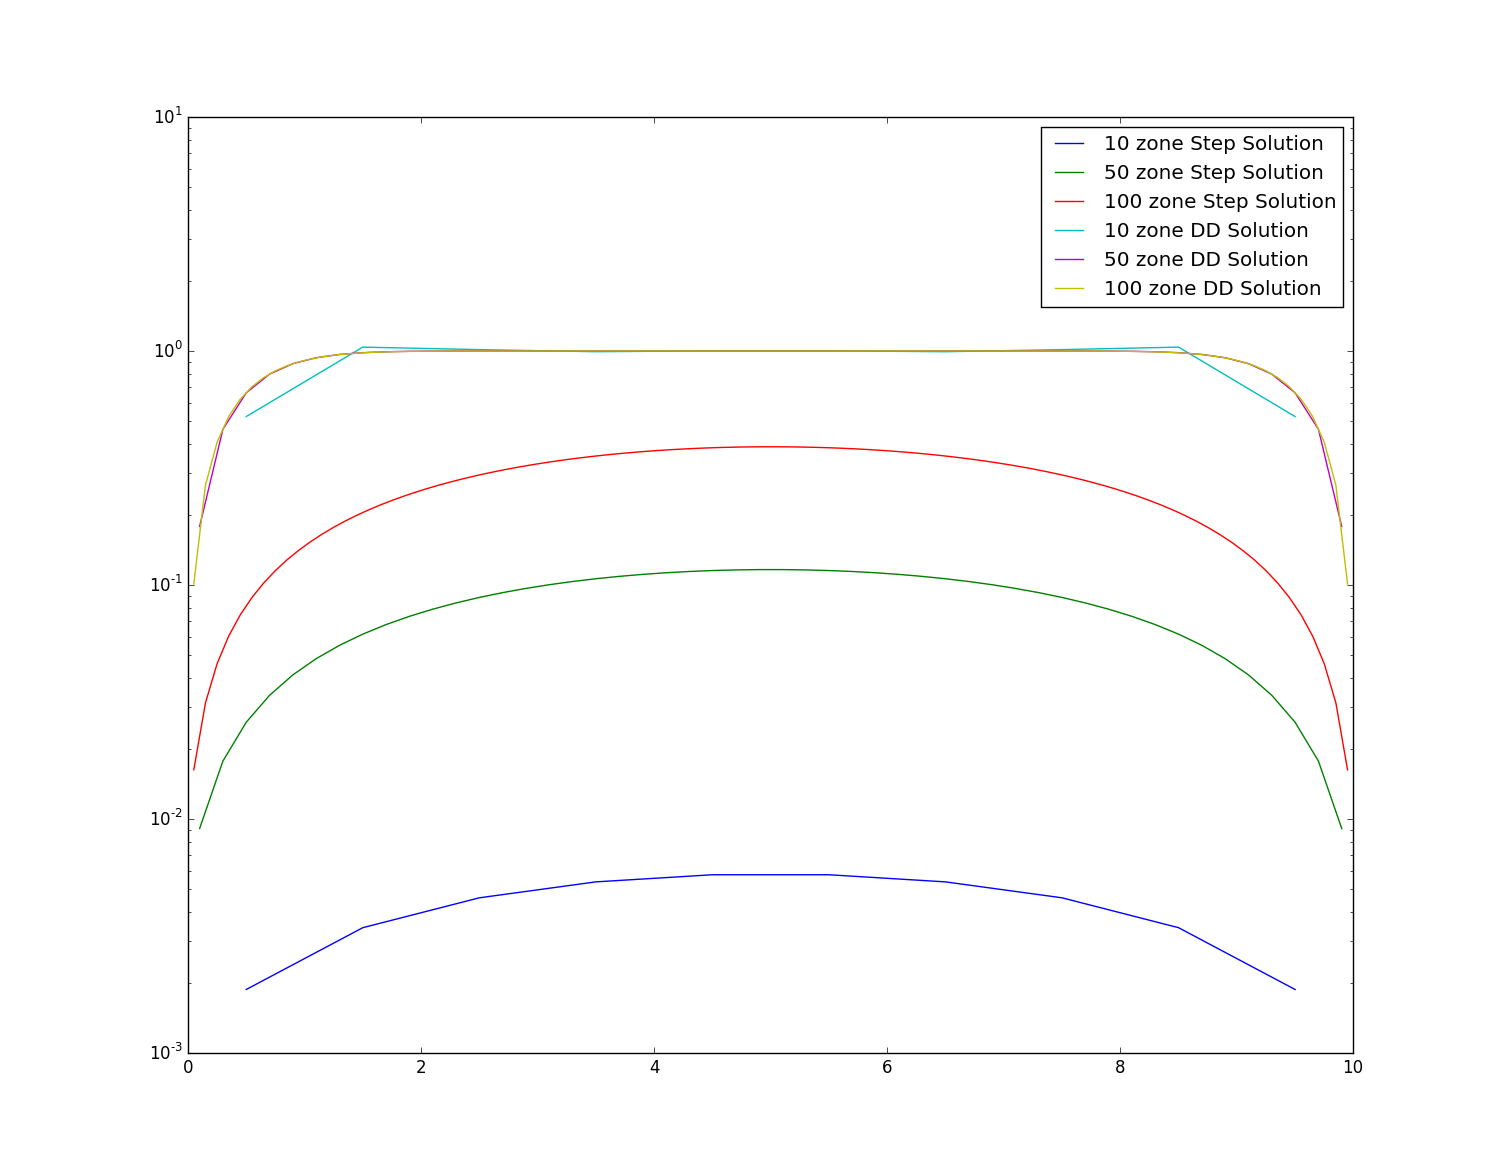
\includegraphics[width=.65\textwidth]{figures/1_1.png}
	\caption{Source Iteration Solutions}
\end{figure}

Neither spatial discretization method converges for the source iteration solution method for 
the 10000 maximum iterations specified (excepting the 10 zone step discretization, but it doesn't obtain the correct solution), and
in fact, the step solutions seem not to diverge, likely due to the problem being mostly
dominated by scattering, thus taking the problem further into the diffusion limit in which the step
method does not converge.

\begin{figure}[h!]
	\centering
		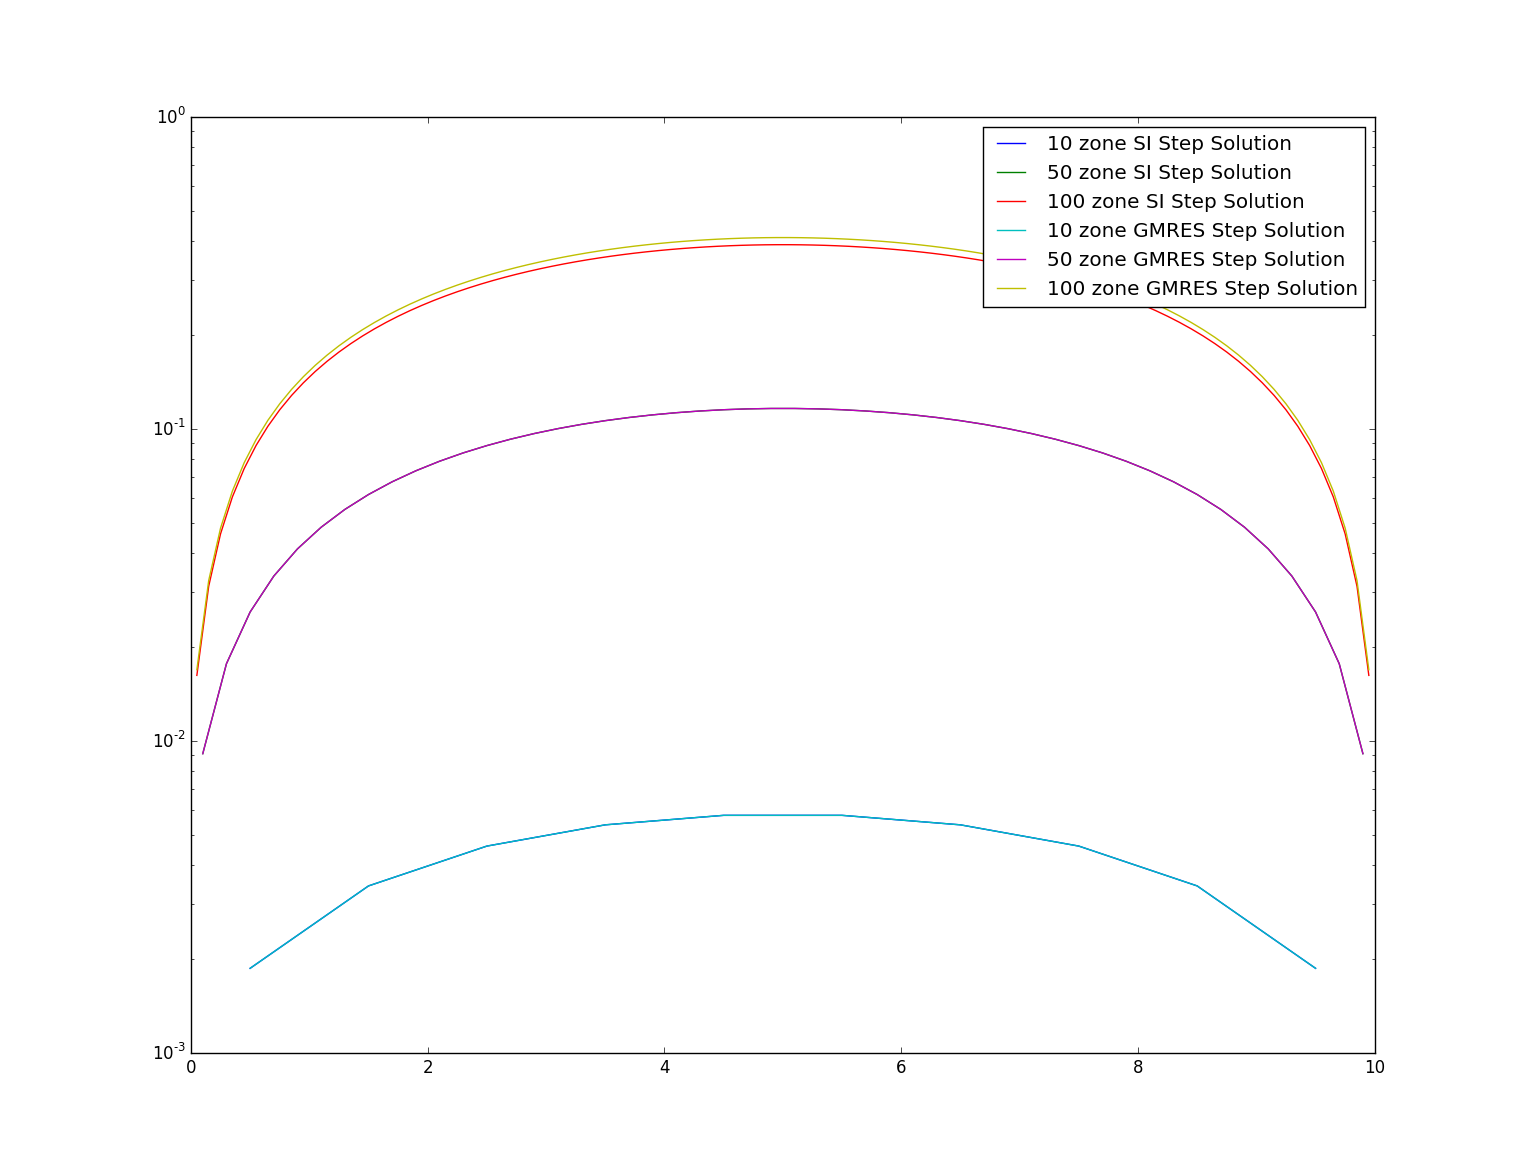
\includegraphics[width=.65\textwidth]{figures/1_2.png}
	\caption{Step Sweep Method Solutions}
\end{figure}

The GMRES and source iteration method solutions overlap in Figure 2 even with the GMRES solution
converging fairly quickly.  This demonstrates that regardless of solution method, the step discretization
is not appropriate to use for problems with a lot of scattering. 

\begin{figure}[h!]
	\centering
		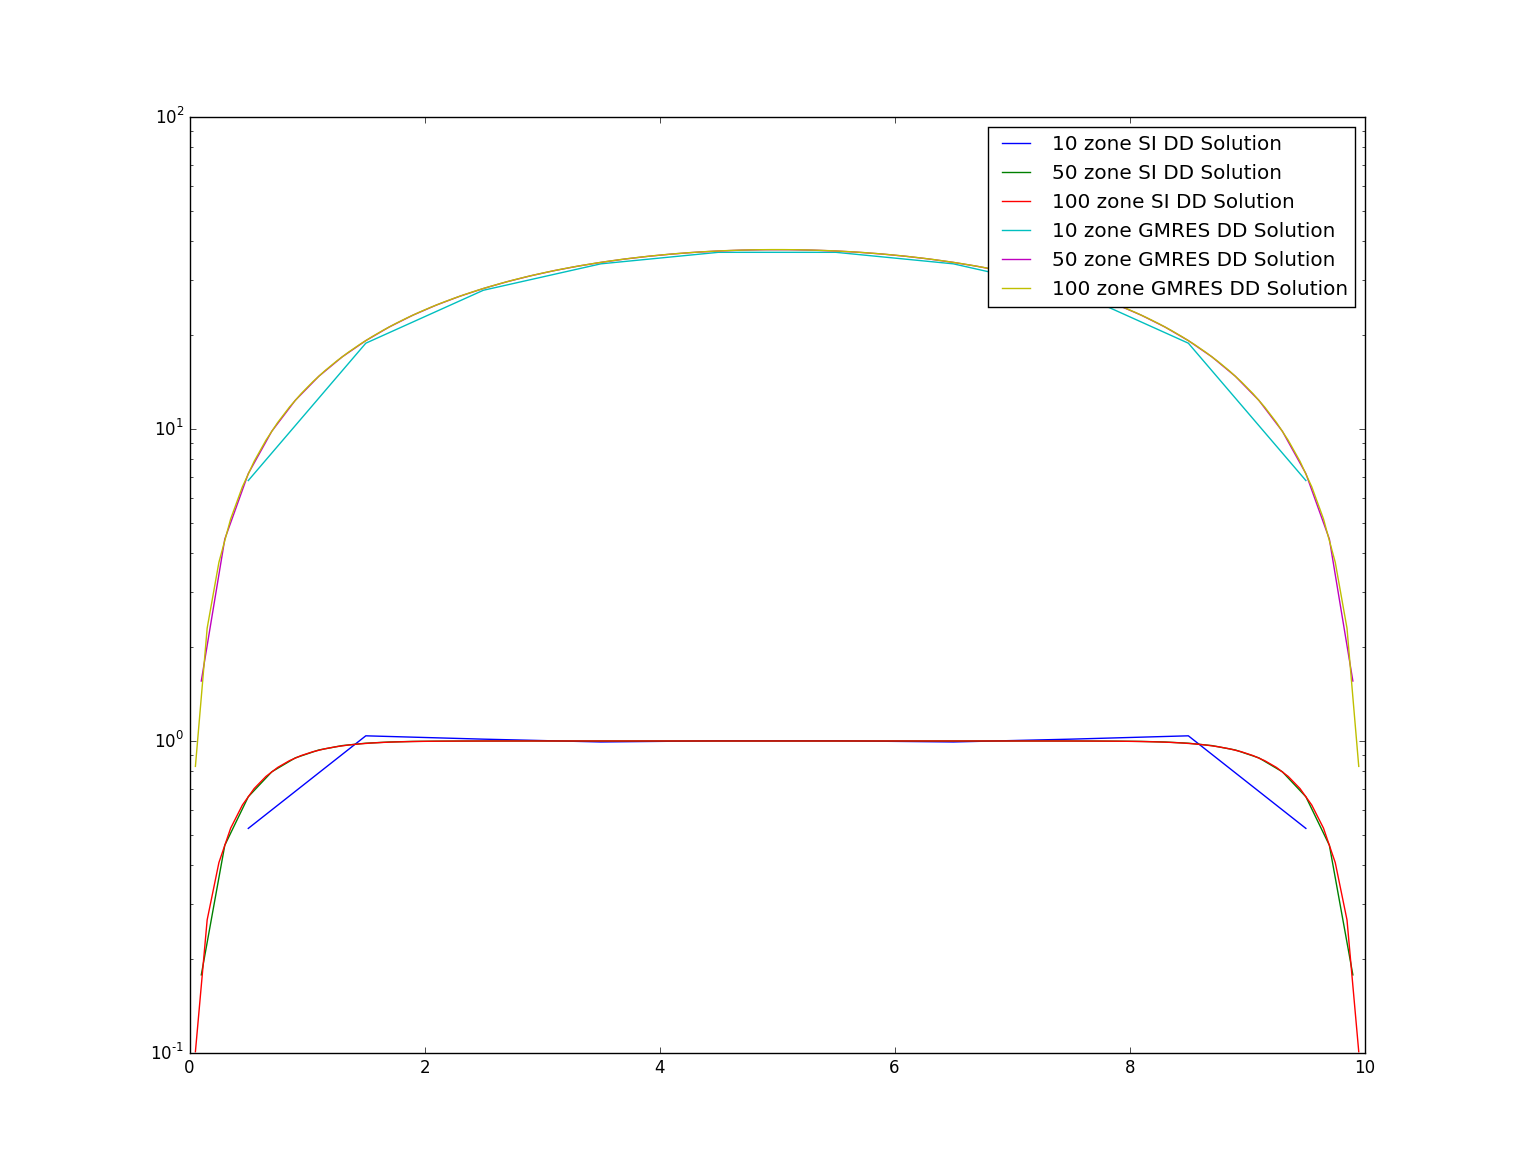
\includegraphics[width=.65\textwidth]{figures/1_3.png}
	\caption{Diamond Difference Method Solutions}
\end{figure}

The diamond difference solutions are interesting in that it looks like we obtain false convergence 
with source iteration (the GMRES solutions converge), but as the source iteration method has not 
converged in any of the spatial resolutions, the solutions end up getting closer to the results obtained
with GMRES the more iterations the source iteration solves are allowed to go through.  

\clearpage

\subsection{2. Difference in Discretizations of Angles}

The two forms of the discretizations for step and diamond difference depending upon the angle arise from 
the direction that the sweep proceeds towards.  Each sweep needs a value from the previous zone; so if the 
sweep is moving in the positive direction originates with the left boundary condition while a sweep in the 
negative direction requires starting with the right boundary condition.  Depending upon the angle from 
quadrature in which the sweep is moving, one discretization is used over the other seeing as no solution 
could be obtained starting at the left boundary and moving in a negative direction or at the right moving
positive.


\subsection{3. Error by Iteration Compared to Source Iteration and GMRES}

\begin{figure}[h!]
	\centering
		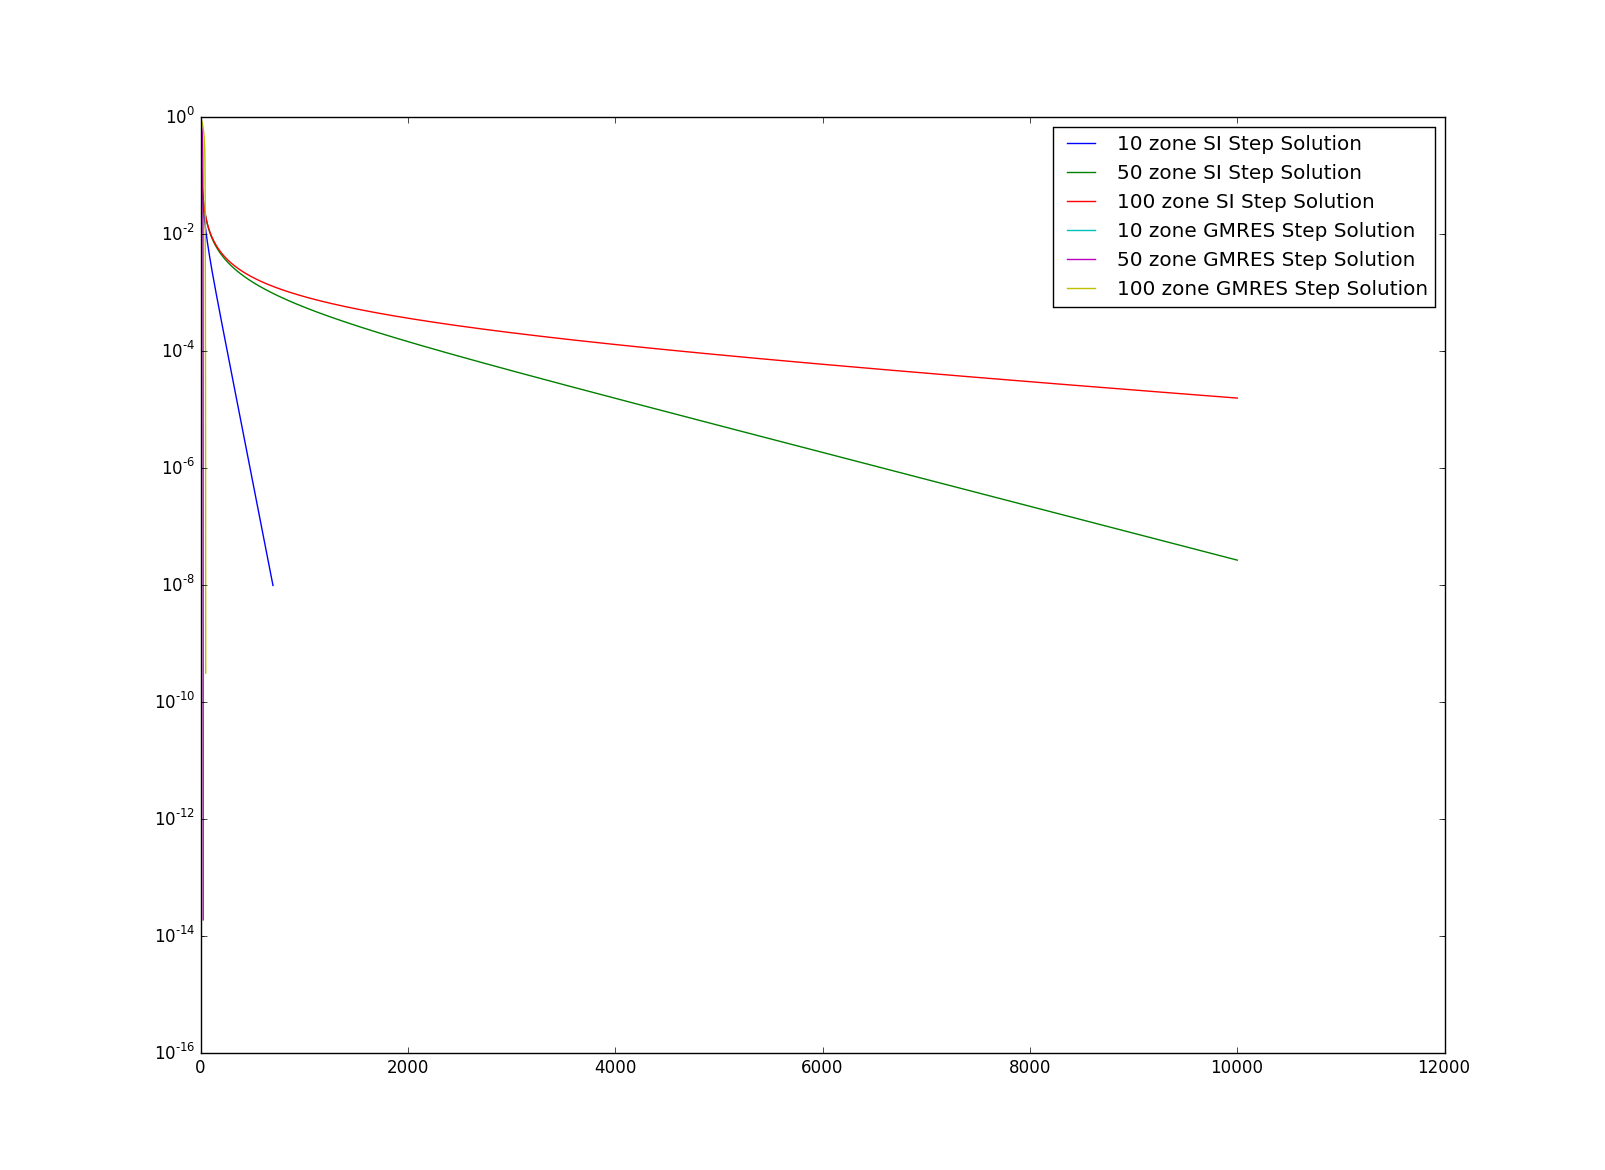
\includegraphics[width=.65\textwidth]{figures/1_4.png}
	\caption{Step Sweep Method Convergence}
\end{figure}

Plotting the convergence of the step sweep discretization, the decrased convergence rate with increased 
spatial resolution is obvious.  Only the 10 zone case converges, and the flux values are too low to be correct
making the method not ideal for the problem.

\clearpage

\begin{figure}[h!]
	\centering
		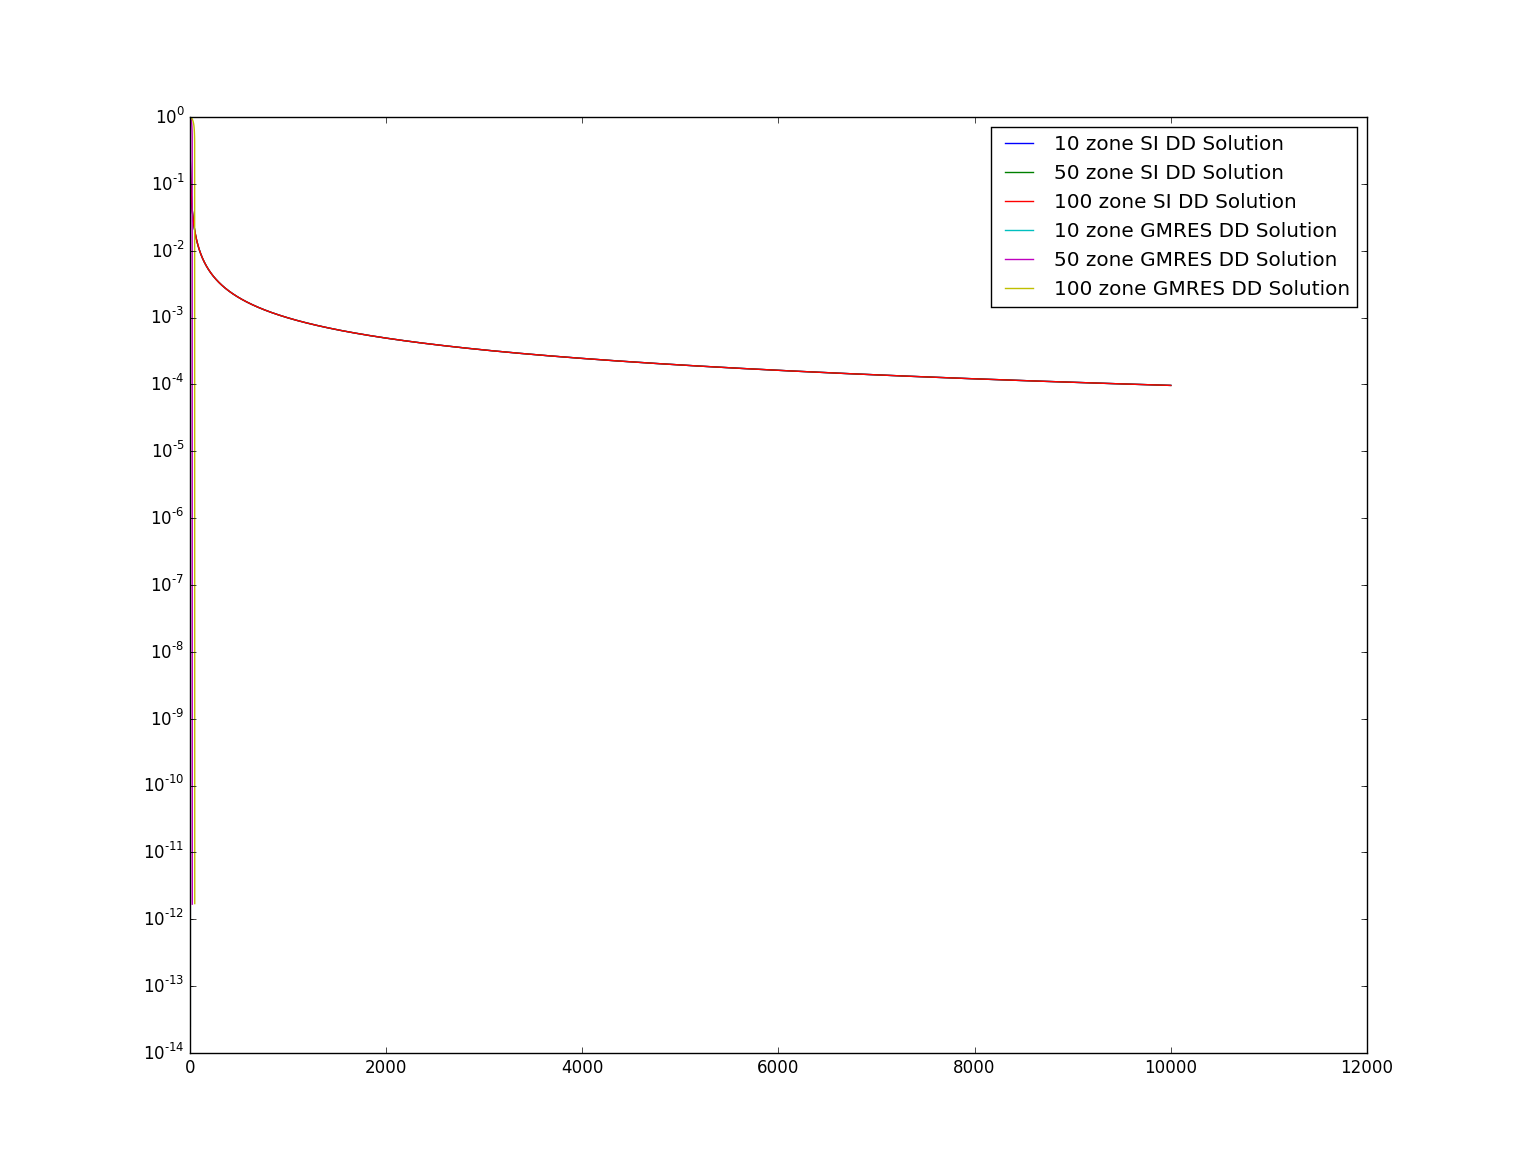
\includegraphics[width=.65\textwidth]{figures/1_5.png}
	\caption{Diamond Difference Method Convergence}
\end{figure}

All of the source iteration diamond difference solutions converge at similar rates, but still extremely slowly
compared to the GMRES method.

\begin{figure}[h!]
	\centering
		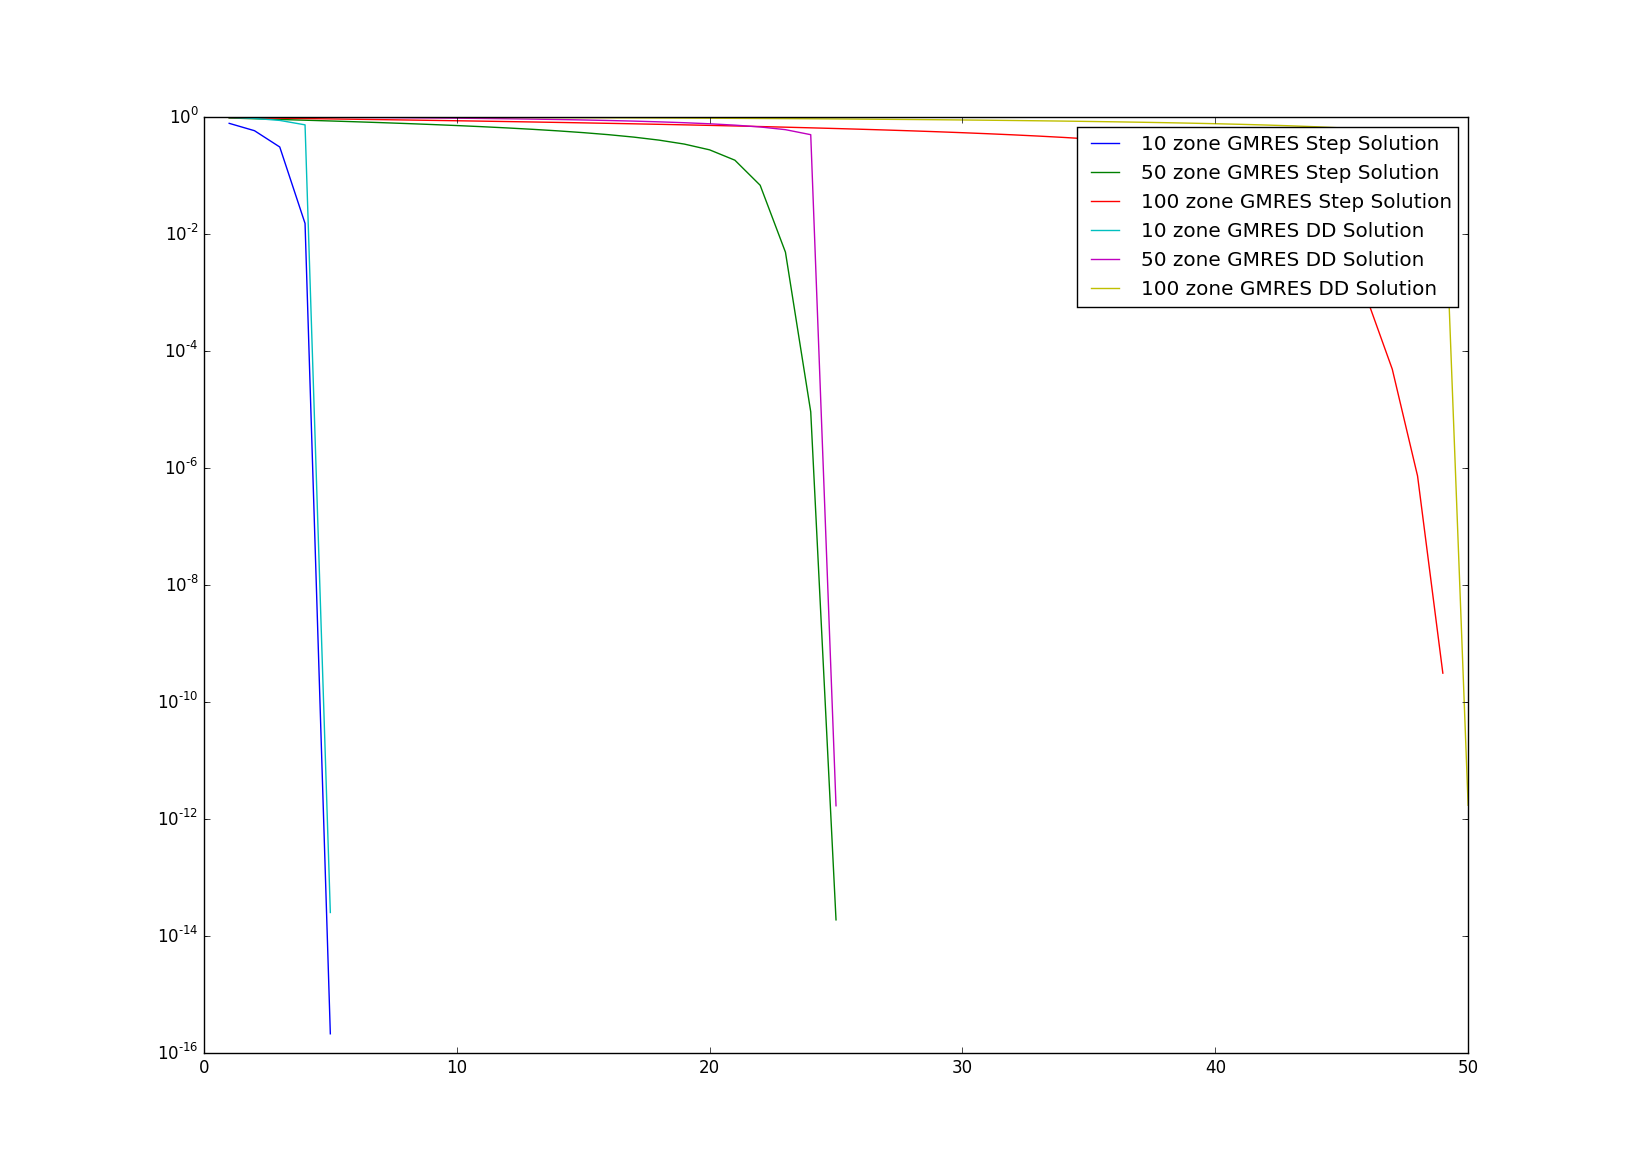
\includegraphics[width=.65\textwidth]{figures/1_6.png}
	\caption{GMRES Convergence}
\end{figure}

Figure 6 is given to compare the GMRES solutions' convergence.  An interesting feature to note for the 
GMRES diamond difference error is that the rate beings slowly, then in one or two iterations quickly converges to the solution
by reducing the error several orders of magnitude.  The GMRES step solutions are more gradual, but again, the method is not
sound for this problem.

\clearpage

\subsection{4. Reed's Problem}

Reed's problem is a benchmark originally devised to test differencing schemes for discrete ordinates codes.
It consists of four mirrored material regions, non-uniform source distribution, and vacuum boundaries (or
depending upon how the problem is set up, a reflecting boundary in the middle).  Using the methods outlined
in the first section of the problem, we are tasked with obtaining and comparing solutions to this problem.

\begin{figure}[h!]
	\centering
		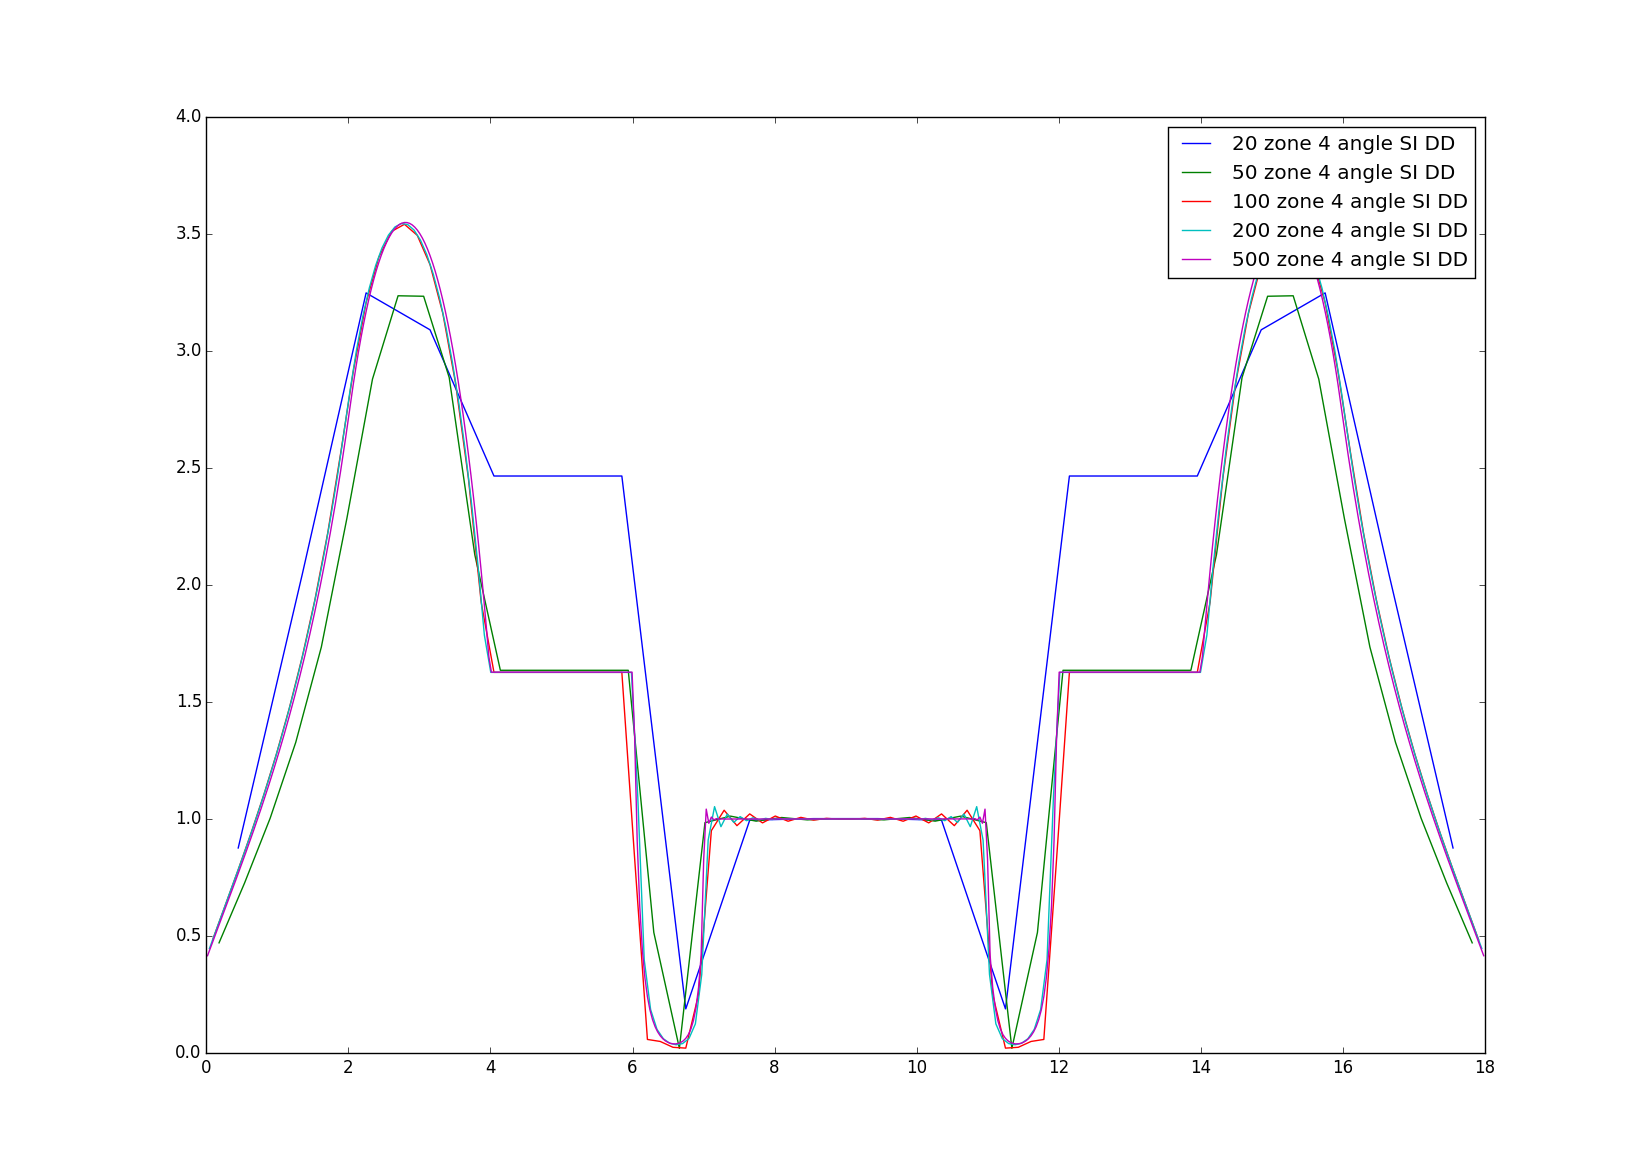
\includegraphics[width=.65\textwidth]{figures/4_1.png}
	\caption{Source Iteration Diamond Difference Solutions with increasing spatial resolution}
\end{figure}

\begin{figure}[h!]
	\centering
		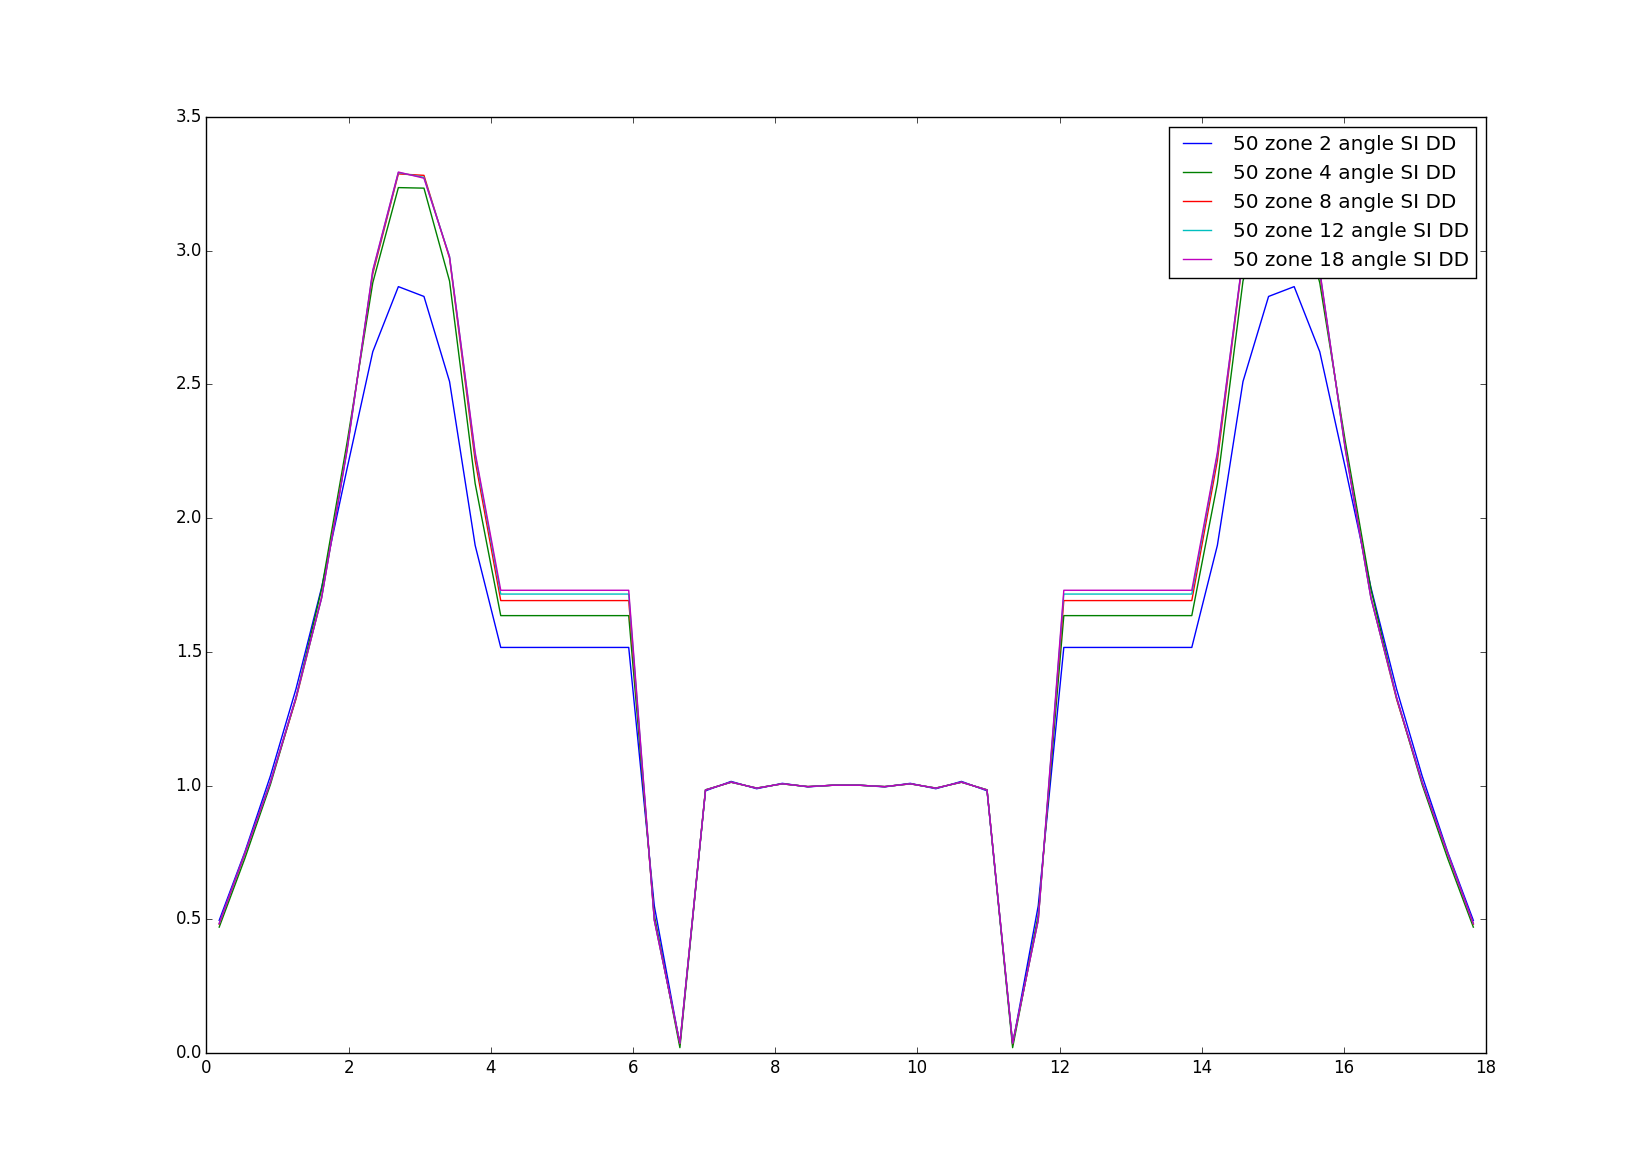
\includegraphics[width=.65\textwidth]{figures/4_2.png}
	\caption{Source Iteration Diamond Difference Solutions with increasing angular resolution}
\end{figure}

\clearpage

\begin{figure}[h!]
	\centering
		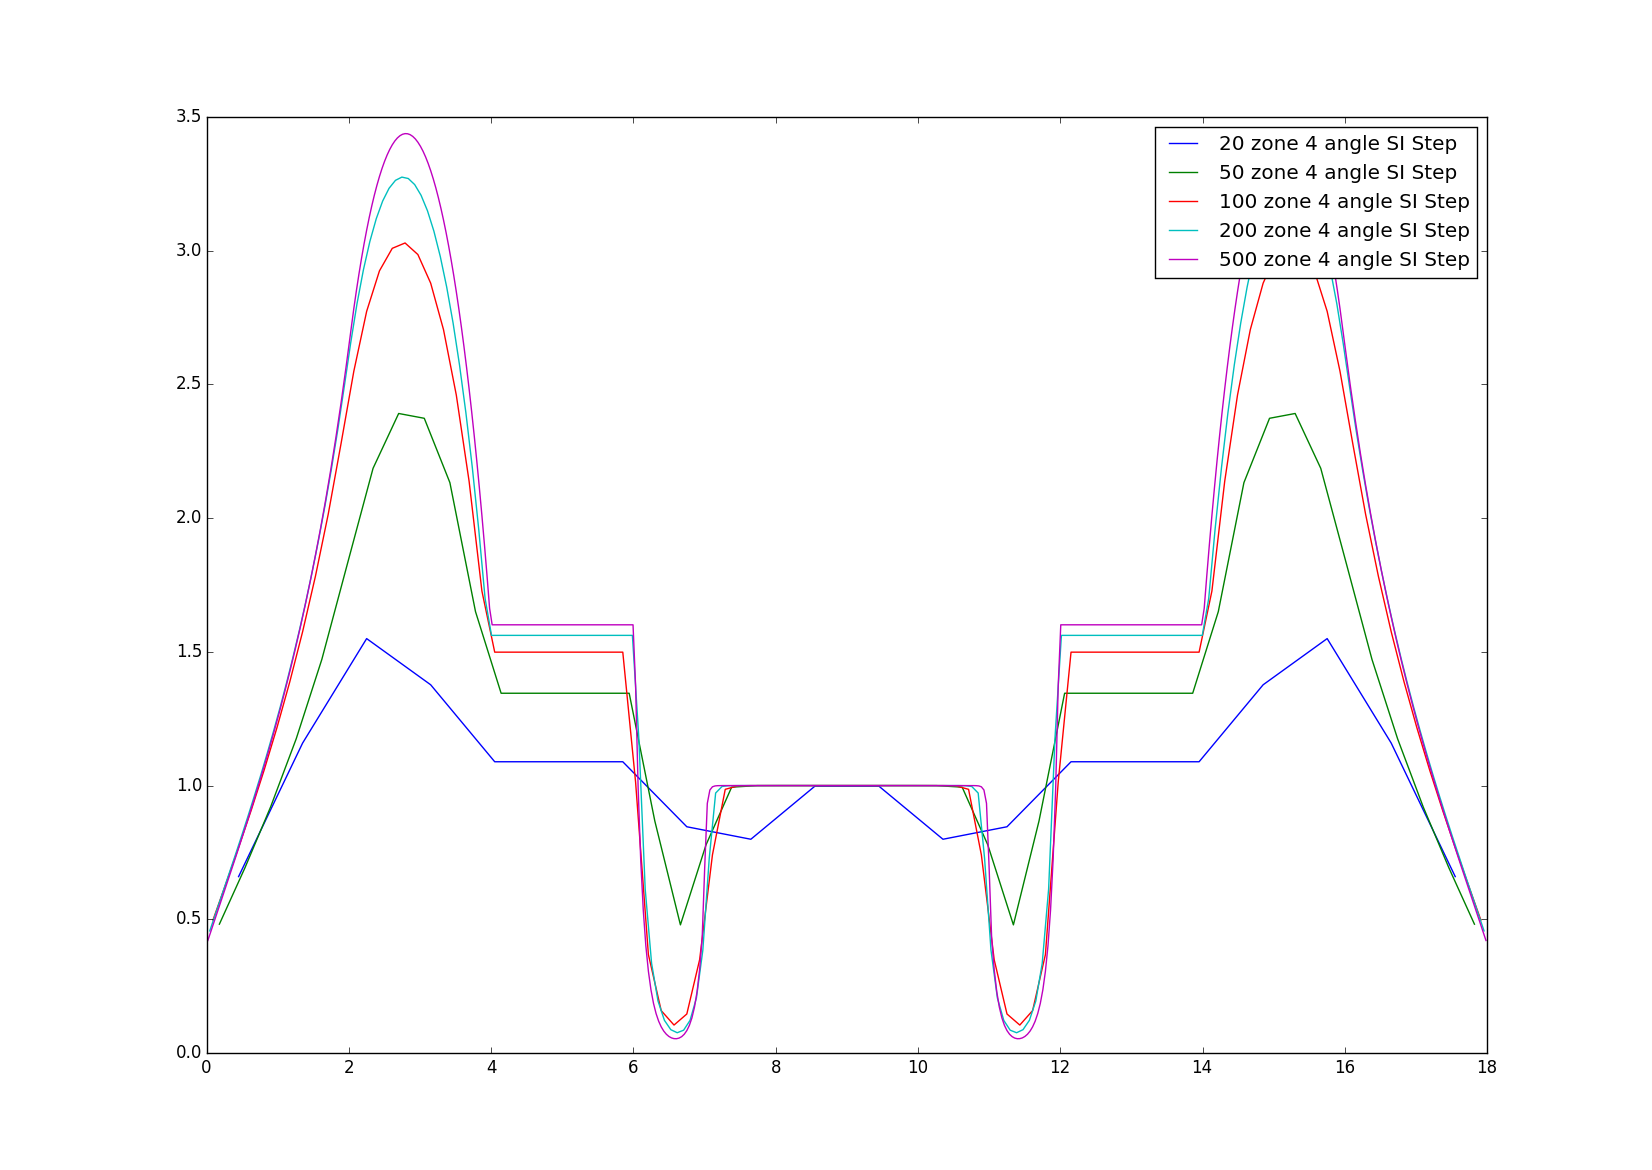
\includegraphics[width=.65\textwidth]{figures/4_3.png}
	\caption{Source Iteration Step Solutions with increasing spatial resolution}
\end{figure}

\begin{figure}[h!]
	\centering
		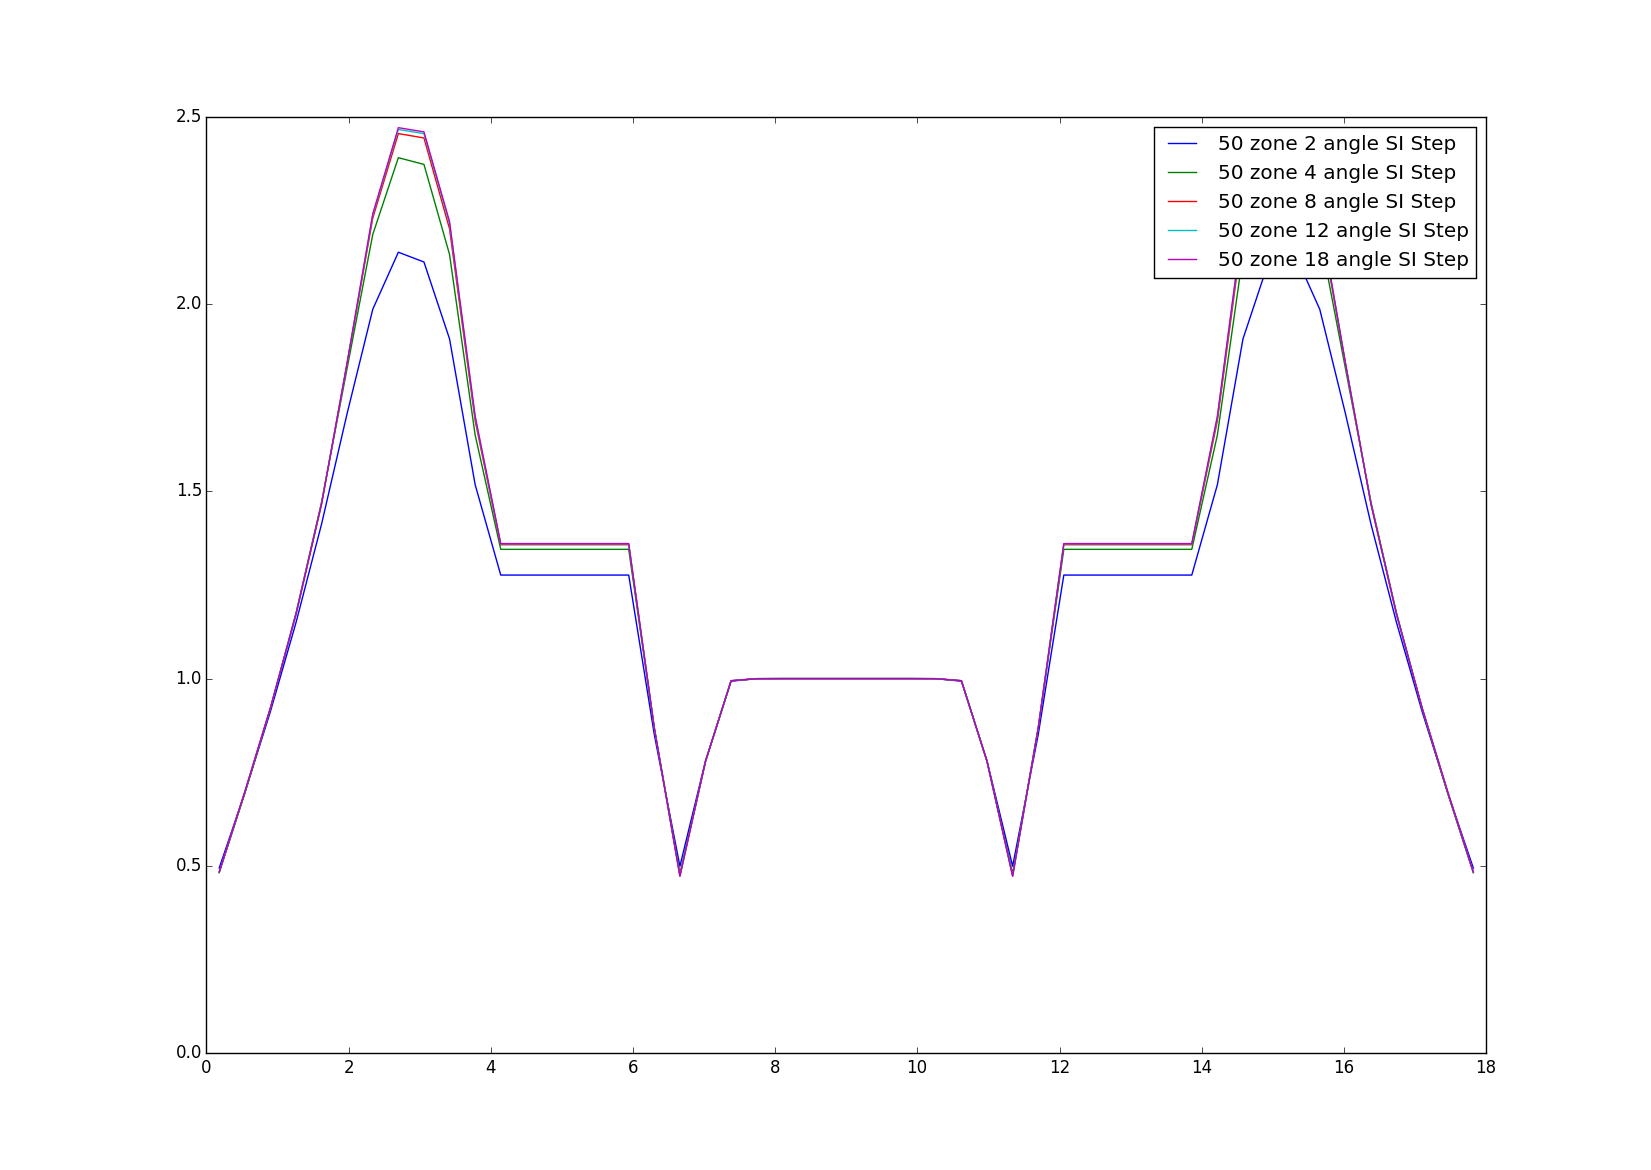
\includegraphics[width=.65\textwidth]{figures/4_4.png}
	\caption{Source Iteration Step Solutions with increasing angular resolution}
\end{figure}

\clearpage

\begin{figure}[h!]
	\centering
		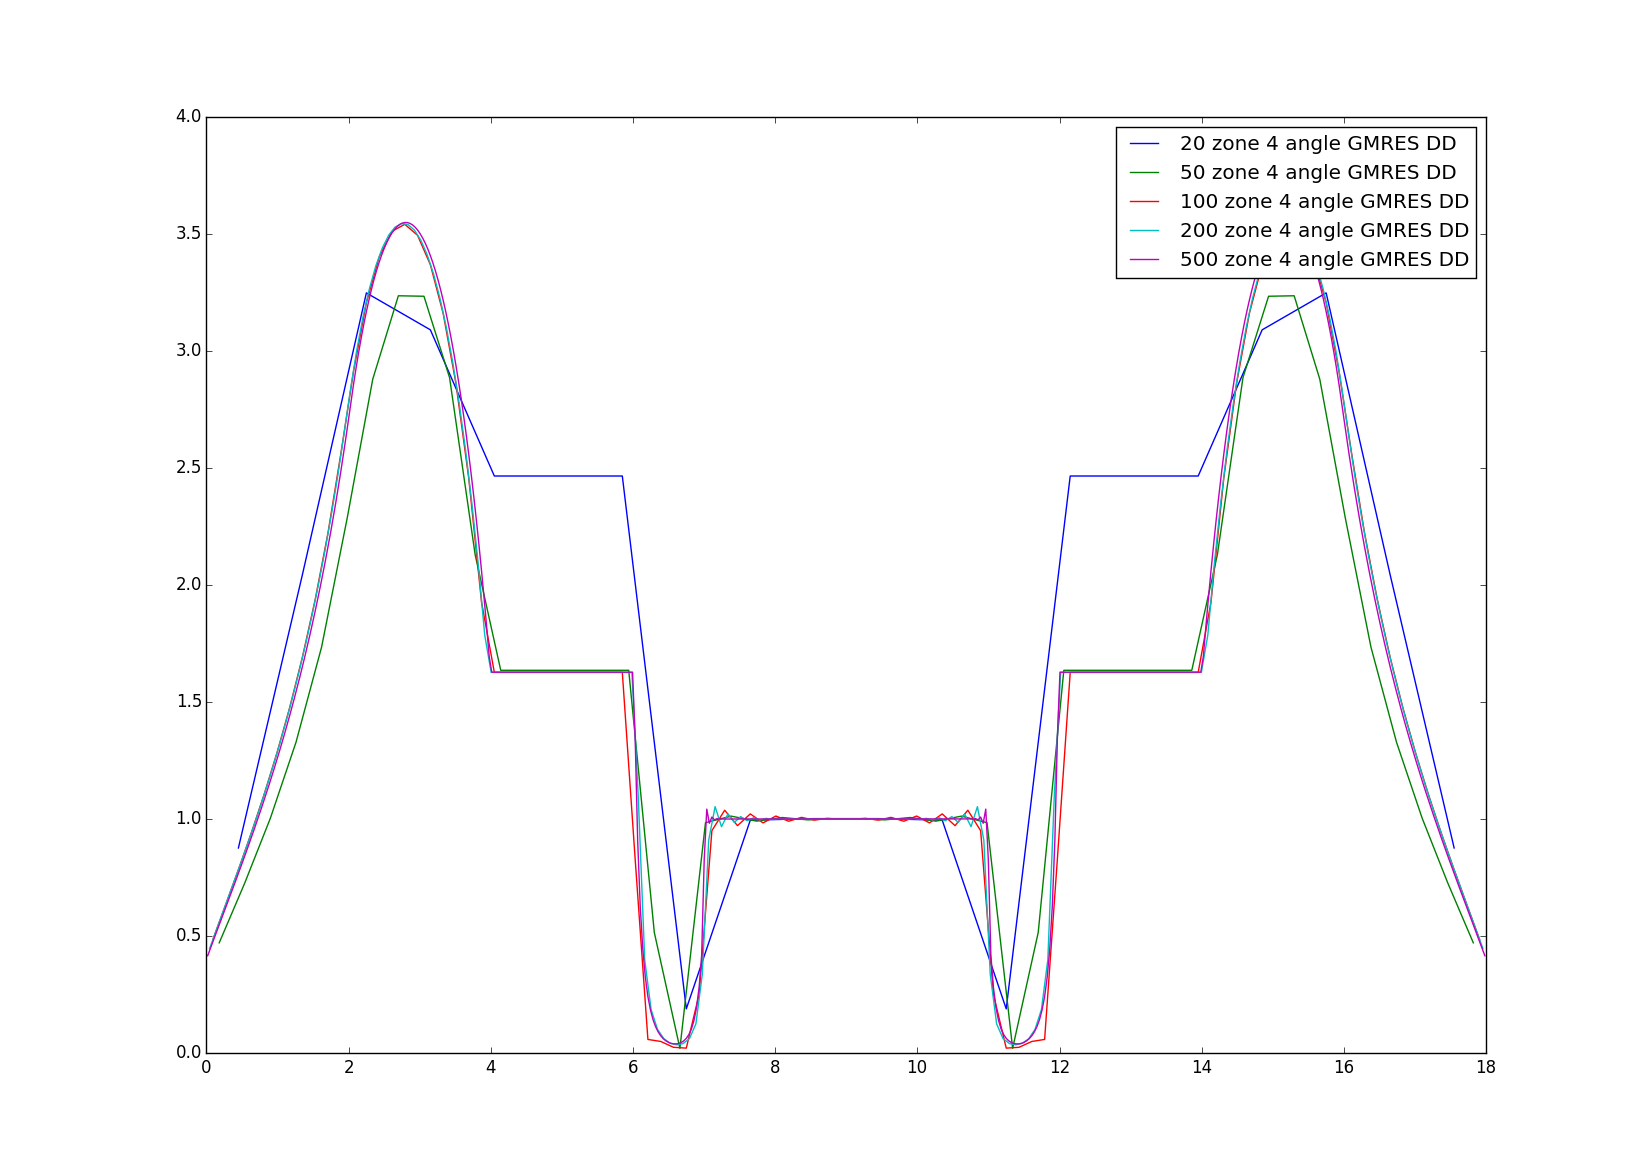
\includegraphics[width=.65\textwidth]{figures/4_5.png}
	\caption{GMRES Diamond Difference Solutions with increasing spatial resolution}
\end{figure}

\begin{figure}[h!]
	\centering
		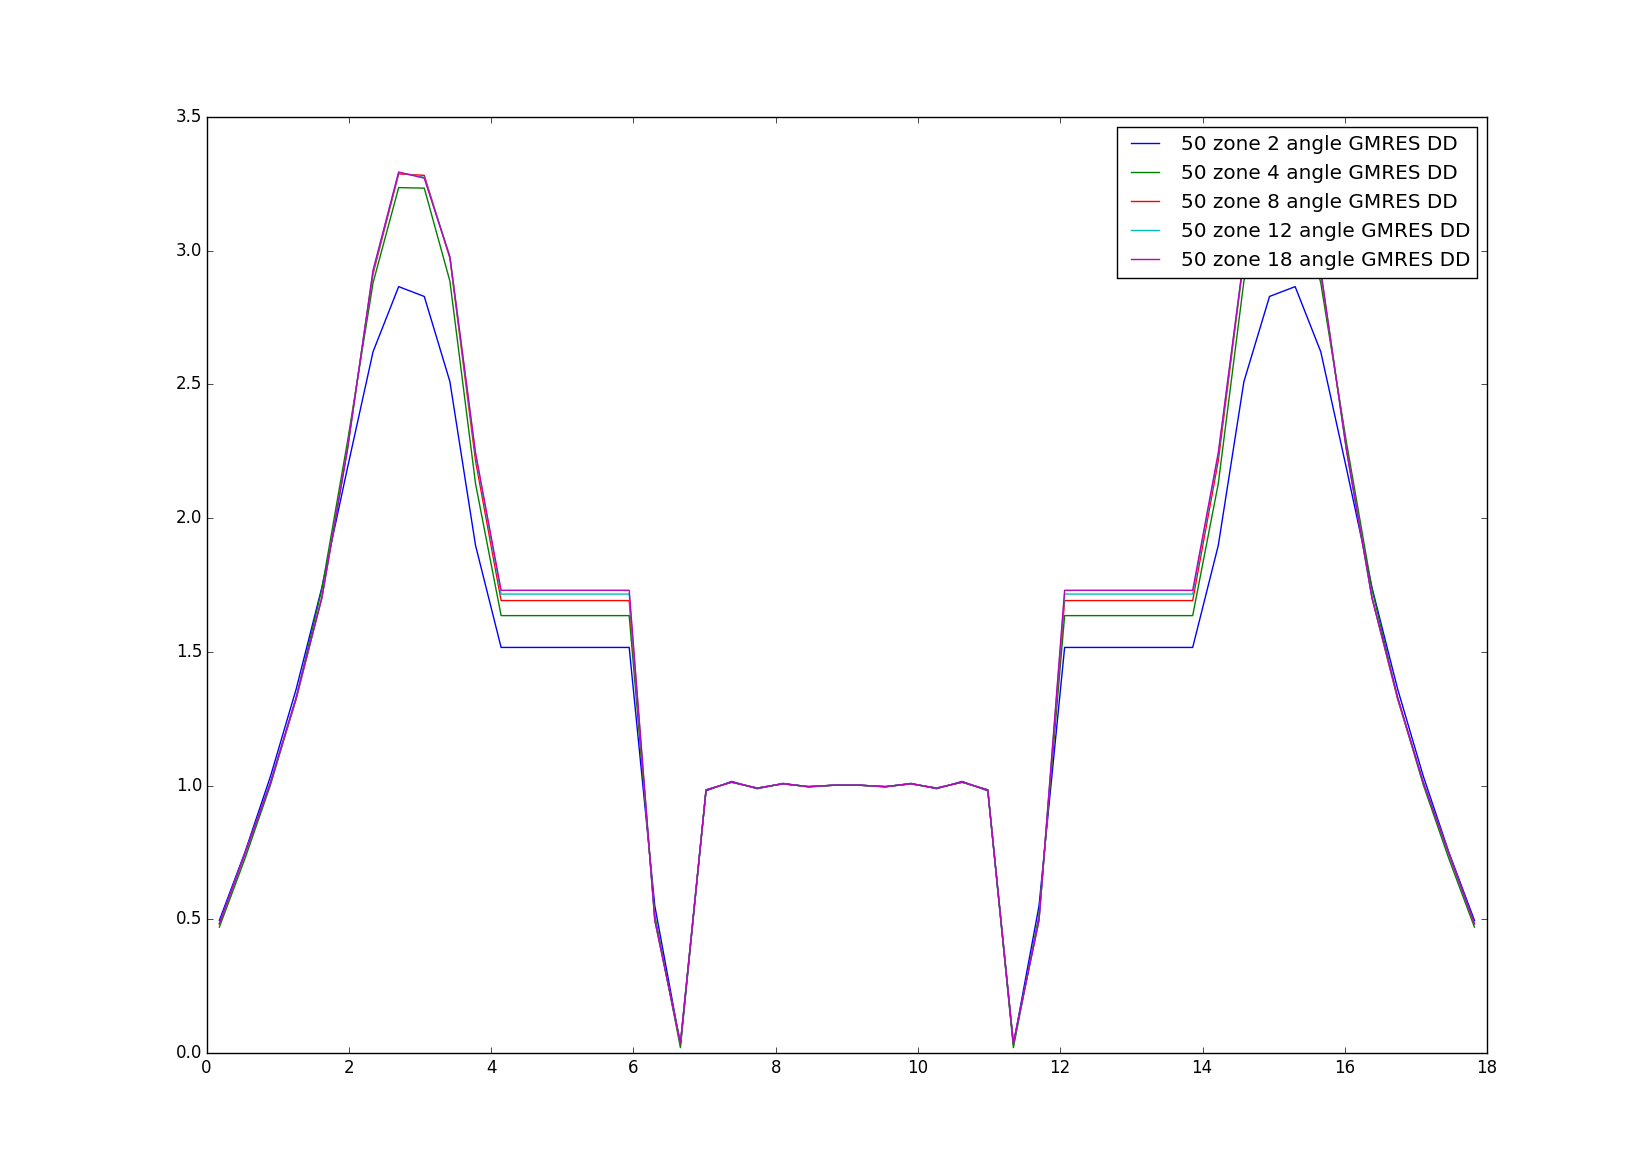
\includegraphics[width=.65\textwidth]{figures/4_6.png}
	\caption{GMRES Diamond Difference Solutions with increasing angular resolution}
\end{figure}

\clearpage

\begin{figure}[h!]
	\centering
		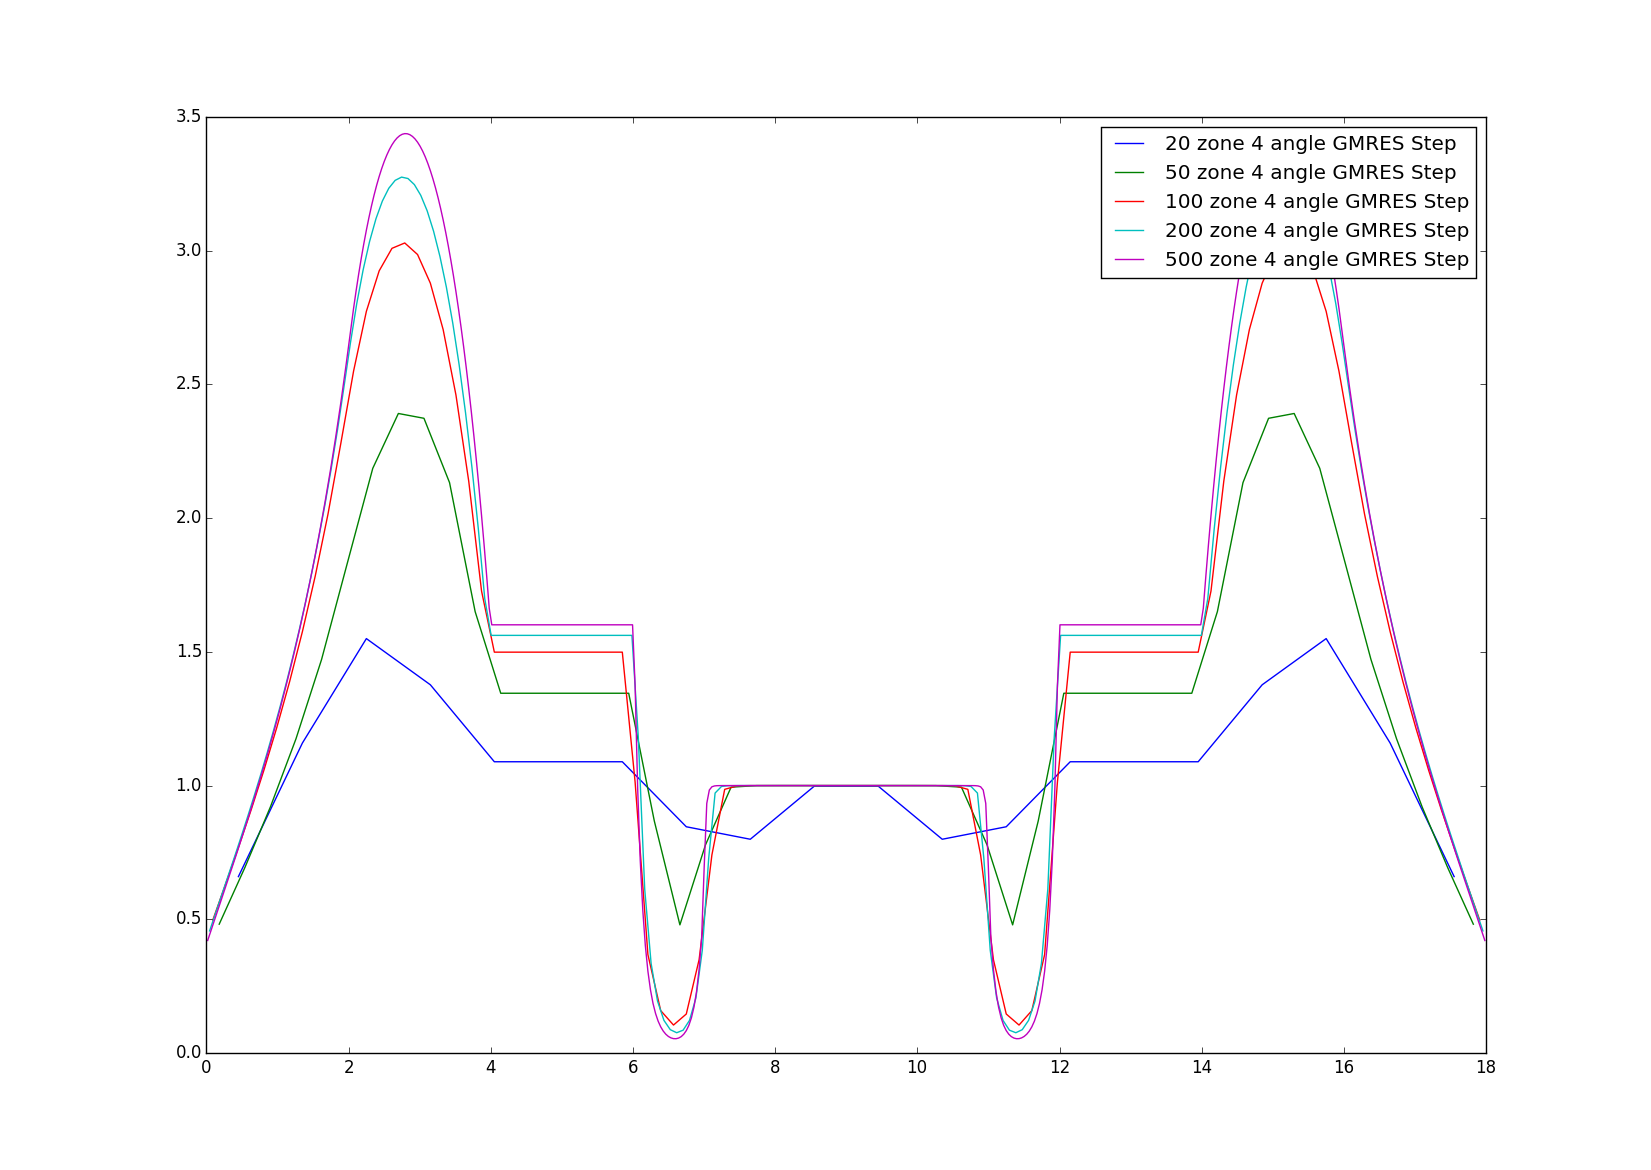
\includegraphics[width=.65\textwidth]{figures/4_7.png}
	\caption{GMRES Step Solutions with increasing spatial resolution}
\end{figure}

\begin{figure}[h!]
	\centering
		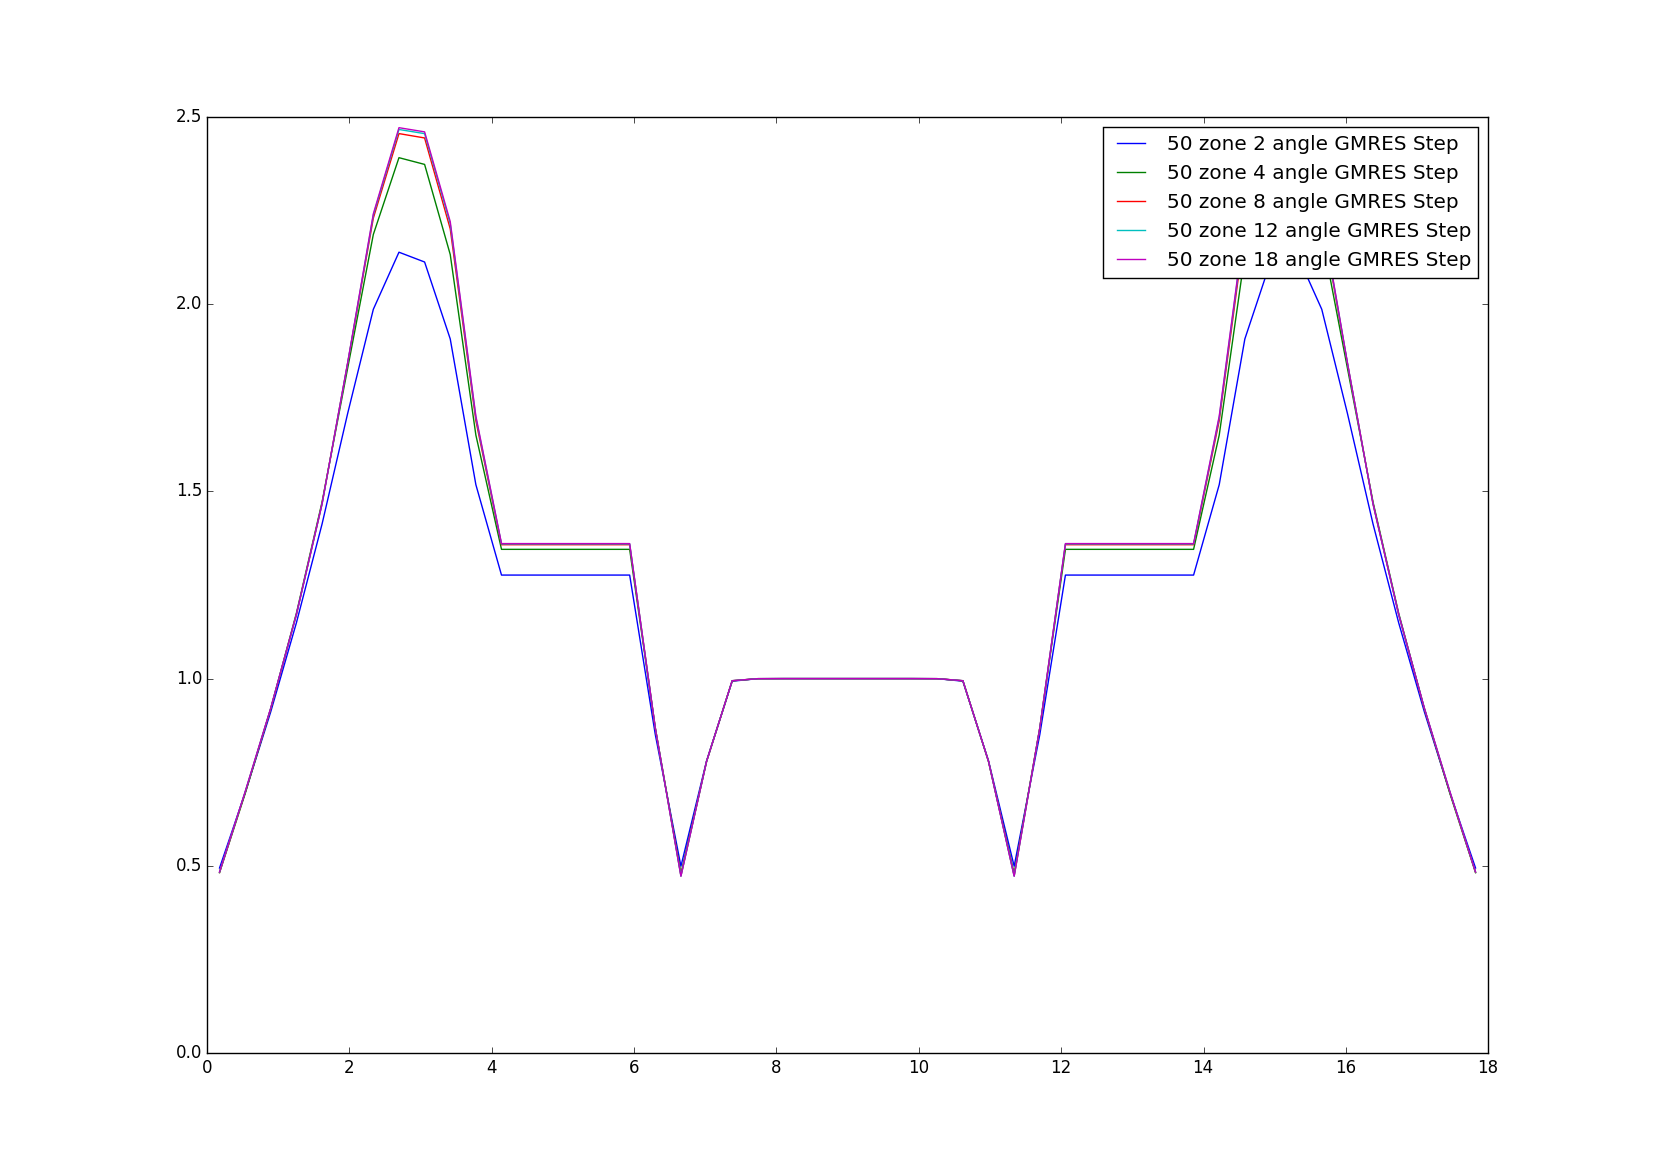
\includegraphics[width=.65\textwidth]{figures/4_8.png}
	\caption{GMRES Step Solutions with increasing angular resolution}
\end{figure}

Unlike the previous problem solved, all methods converge to a solution with Reed's problem.  A few features 
of the solutions stand out for the various methods when increasing the spatial and angular resolution.  The
diamond difference method seems to contain spatial oscillations in the center region that increased spatial resolution
mitigates.  Step solution methods start out as fairly bad approximations of the solution, but quickly converge with 
increased spatial resolution.  It appears that increasing the number of angles in the quadrature scales the solution
closer to the true evaluation, but this problem looks more spatially dependent.

\clearpage

\begin{figure}[h!]
	\centering
		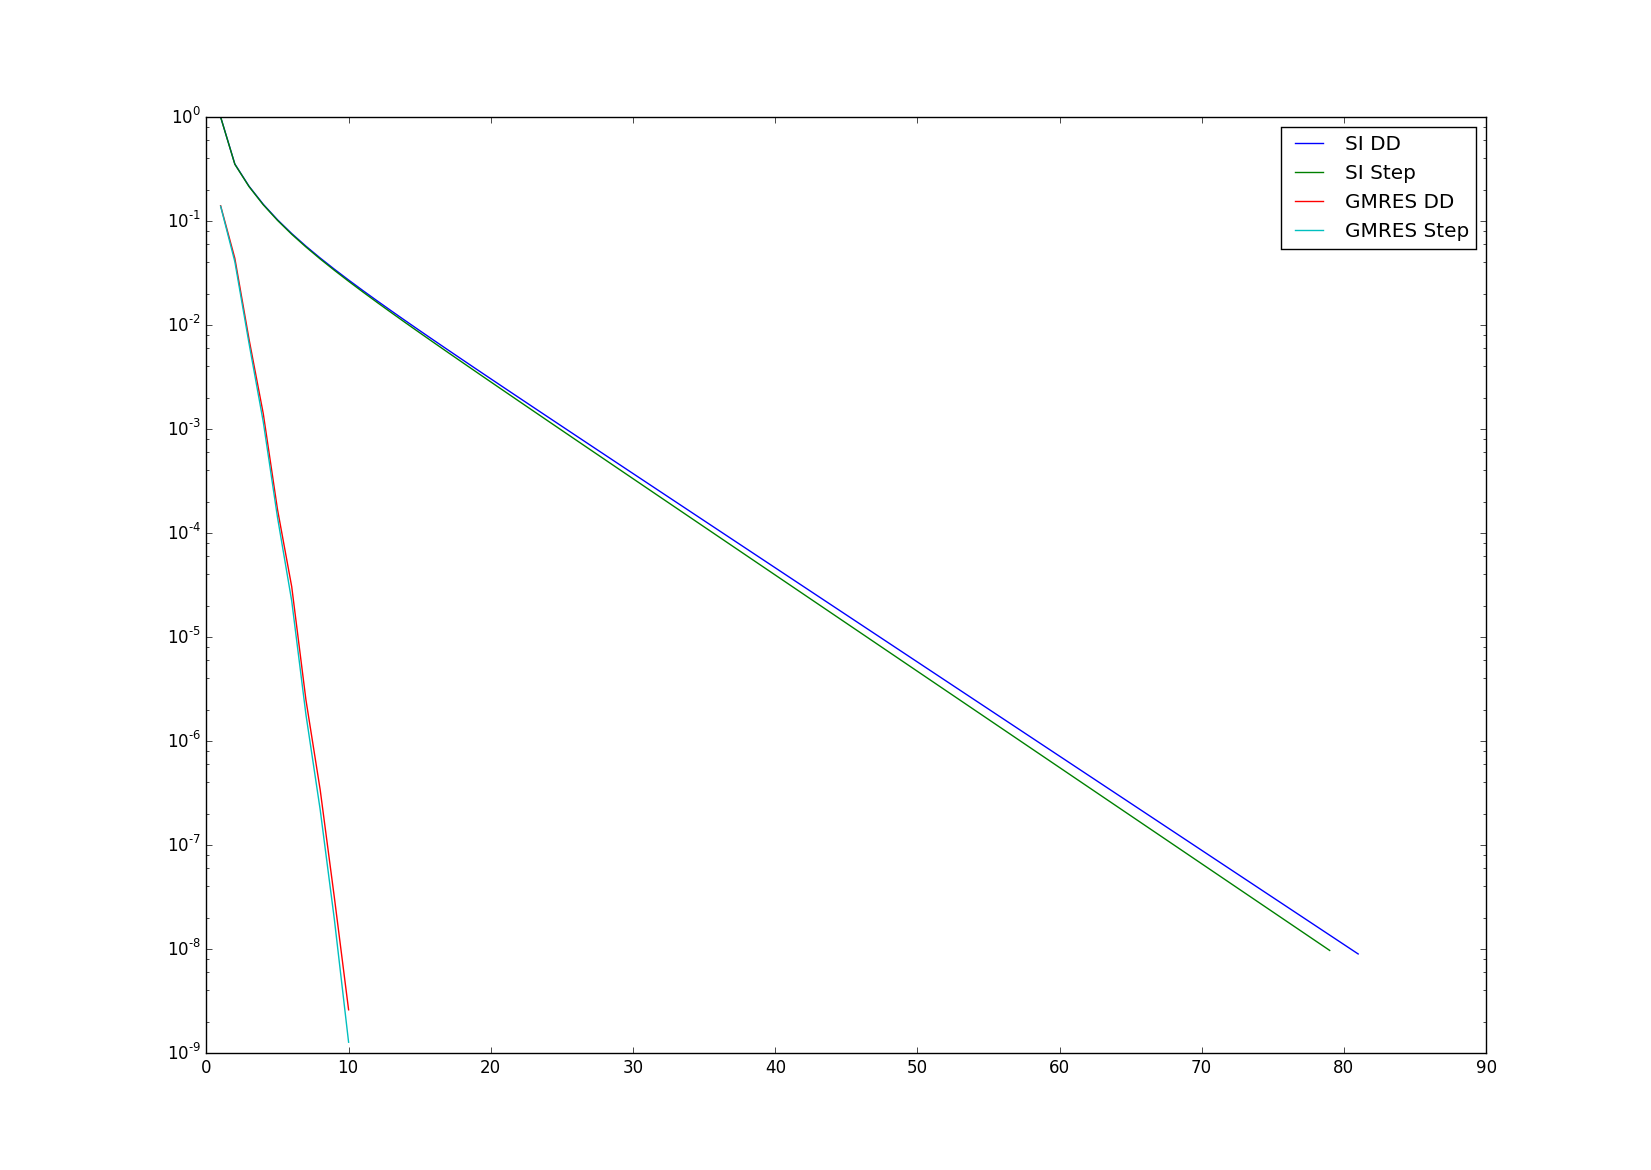
\includegraphics[width=.65\textwidth]{figures/4_9.png}
	\caption{Convergence of solution methods for highest spatial and angular resolution}
\end{figure}

GMRES converges much faster than source iteration for this problem and the step method 
converges faster than diamond difference in this problem due to the reduced amount of scattering
compared to the previous problem.

\end{homeworkProblem}

\end{document}